\chapter{Pumpelemmaet for regulære og kontekstfrie sprog}

\section{Pumpelemmaet for Regulære Sprog}%
\label{sec:pumpinglemmarl}

Der er nogle sprog der ikke er regulære. Givet et specifikt sprog, kan vi bevise om det er, eller ikke er, regulært ved brug af \textit{pumpelemmaet}.

\begin{theorem}[Pumpelemmaet]
	Lad $A$ være et regulært sprog over \(\Sigma\). Så eksisterer der et $p \in \mathbb{N}$ hvor \(\forall s \in A\) hvor $|s| \ge p$, så kan det opdeles $s = xyz$ hvor $x,y,z \in \Sigma^{*}$. Ved denne gælder følgende betinglser:
	\begin{enumerate}
		\item $xy^{i}z \in A \; \forall i \ge 0$: $y$-delen skal kunne ``pumpes''.
		\item $|y| > 0$: $y$-delen må ikke være $\varepsilon$.
		\item $|xy| \le p$: $xy$ delen skal højest have længde $p$.
	\end{enumerate}
\end{theorem}

Før vi går til beviset, bemærk at denne sætning udelukkende gælder ved uendelige sprog. Dette er fordi \textit{alle endelige sprog er regulære.} Givet et sprog der indeholder strenge $w_{1}, w_{2}, \ldots, w_{n}$, lav en endelig automat der accepterer hhv. $w_{1}, w_{2}, \ldots, w_{n}$ og lav foreningsmængde på dem, for at få en endelig automat der accepterer dem alle, i.e. hele sproget.

\begin{proof}
	Lad $M$ være en DFA hvor $L(M) = A$ og lad $p = $ antallet af tilstnade i $M$.
	Siden $|s| \ge p$ må mindst én tilstand af $M$ gentages mindst én gang imens $M$ læser $s$. Bemærk at $|s|$ kan være lig $p$, da det først er ved tilstanden efter starttilstanden, at læsningen af $s$ begynder. Dette kommer fra dueslagsprincippet.

	Lad $q$ være den første tilstand som bliver gentaget da $M$ læser $s$.

	\begin{center}
		\begin{tikzpicture}
			\node[state, initial] (q0) at (0,0) {$q_0$};
			\node[state, right of=q0] (q) {$q$};
			\node[state, accepting, right of=q] (qacc) {$q_{acc}$};

			\draw  (q0) edge node{$x$} (q)
			(q) edge[loop above] node{$y$} (q)
			(q) edge node{$z$} (qacc);

		\end{tikzpicture}
	\end{center}
	Vi vil nu vise hvorfor hver af de 3 betingelser fra sætningen holder:

	\begin{enumerate}
		\item Det holder at vi kan gentage $y$ så mange gange vi har lyst til, og endda helt undgå at bruge $y$ (i sådan et tilfælde ville løkken fra $q$ til $q$ naturligvis være redundant).
		\item Denne holder, da vi skal læse mindst én symbol, ellers ville $|s| = p-1$.
		\item Denne holder fordi $q$ er den første tilstand vi ser mere end én gang.
	\end{enumerate}
\end{proof}

\subsection{Hvordan man bruger pumpelemmaet}%
\label{subsec:label}

Hovedårsagen til at vi lærer om pumpelemmaet, er for at kunne bevise hvorvidt et sprog er regulært eller ej. Vi bruger i sådan et tilfælde pumpelemmaet i et modstridsbevis, hvor vi antager at et sprog er regulært, og beviser derefter at dette \textit{ikke} kan passe.

Generelt fungerer processen som følger (Tager fra Jørgens noter, 21 minutter inde i video 2):
\begin{itemize}
	\item Antag at $L$ er regulært
	\item Lad $L = L(M)$ for en DFA $M$. Lad $P$ være antallet af tilstande i $M$.
	\item Vi vælger en streng $s \in L$ hvor $|s| \ge p$
	\item Modstanderen giver en $s = xyz$ der opfylder 2. og 3. betingelse i pumpelemmaet.
	\item Vi finder en værdi $i$ hvor 1. betingelse i pumpelemmaet ikke holder, hvilket giver et modstrid.
\end{itemize}

Hvis det er muligt at bevise at hverken 2. eller 3. betingelse nogensinde kan holde, er dette også en måde at bevise nonregulæritet på.

Vi kigger på et eksempel, med det måske mest populære nonregulære sprog: $B = \{0^{n}1^{n} \mid n \ge 0\}$. Processen for at bevise dennes nonregulæritet er som følger:
\begin{itemize}
	\item Antag at $B$ er regulært. Lad $M$ være en DFA med $L(M) = B$ og lad $p$ være antallet af tilstande af $m$.
	\item Vi vælger strengen $s = 0^{p}1^{p}$
	\item Modstanderen foreslår opdeling $s = xyz$ som opretholder betingelse 2 og 3 i pumpelemmaet, altså $|y| > 0, |xy| \le p$.
	\item Da $|xy| \le p$ har vi at $y = 0^{r}$ for en $r > 0$. Dermed $xz = 0^{p-r}1^{p} \notin B$ hvilket er modstrid for første betingelse af sætningen.
\end{itemize}

En anden måde at bevise på er ved at bruge \textit{closure} egenskaberne.

Vi kigger på ét andet eksempel: $C = \{w \in \{0,1\}^{*} \mid \#_{0}(w) = \#_{1}(w)\}$.
\begin{itemize}
	\item Vi antager at $C$ er regulært og lader $M$ være en DFA hvor $L(M) = C$ og lad $p $ være antallet af tilstande af $M$
	\item Vi vælger $s = 0^{p}1^{p}$
	\item Modstanderne foreslår en $s = xyz$ der opretholder betingelse 2 og 3 fra pumpelemmaet.
	\item Da $|xy| \le p$ må $y = 0^{r}$ for nogen $r > 0$. Dermed $xz = 0^{p-r}1^{p} \notin C$, hvilket er en modstrid.
\end{itemize}

\section{Pumpelemmaet for Kontekstfrie Sprog}%
\label{sec:label}

Præcis ligesom der eksisterer et pumpelemma for regulære sprog, eksisterer der ligeså et for kontekstfrie sprog, der minder meget om. Dette bruges til at bevise nonkontekstfrihed for et sprog.

Disse noter bruger beviset fra Jørgens slides, og \textit{ikke} det fra bogen.

\begin{theorem}[Pumpelemmaet]
	For hvert kontekstfrit sprog $L$ eksisterer der $p \in \mathbb{N}$ således at \(\forall w \in L\) hvor $|w| \ge p$, så kan $w$ deles op $w = uvxyz$ hvor $u,v,x,y,z \in \Sigma^{*}$ og hvor følgende betingelser gælder:
	\begin{enumerate}
		\item $uv^{i}xy^{i}z \in L \; \forall i \ge 0$
		\item $|vy| > 0$
		\item $|vxy| \le p$
	\end{enumerate}
\end{theorem}

\begin{proof}
	Da $L$ er et kontekstfrit sprog, eksisterer der en kontekstfri grammatik $G = (V, \Sigma, R, S)$ i Chomsky Normal Form, i.e., en Chomsky Grammatik, hvor $L = L(G)$.

	Husk tilbage til beviset for pumpelemmaet til regulære sprog, hvor vi lod $p$ være lig med antallet af tilstande. Her lader vi $p = 2^{|V| +1}$ hvor $|V|$ er antallet af variabler. Da det er en Chomsky Grammatik, kan vi se afledning som et parsetræ, hvor hver knude har \textit{højest} to børn. I det sidste skridt af afledningen konvertes en variabel til en terminal. Da $p = 2^{|V|+1}$ er der mindst $2^{|V|+1}$ blade i parsetræet. Disse blade udgører $w$.

	Ud fra dette, er højden på træet \textit{mindst} $|V|+2$, da det sidste skridt er af formen $A_{i} \rightarrow a$. Lad $h(T)$ være højden af $T$; så $h(T) \ge |V|+2$.

	Bemærk nu, at længden af træet er \textit{så} langt at det er \textbf{nødt} til at gentage en variabel. Her ser vi også hvorfor højden af træet skal være $|V|+2$, da hvis det var under (e.g. $|V|+1$) kunne vi have gået $|V|$ variabler igennem, og være sluttet med en transformation til en terminal.

	I Figur~\ref{fig:pumpelemmacfg} ses en grafisk visning af de gentagne variabler.

	Hver af de tre betingelser holder fra dette bevis:
	\begin{enumerate}
		\item $v$ og $y$ kan gentages så meget som muligt, med det gentagne variabel (i vores eksempel var dette $B$).
		\item $|vy| > 0$, fordi hvis $|vy| = 0$ ville $p < 2^{|V|+1}$.
		\item $|vxy| \le p$, da, hvis $|xxy| > p$ ville parsetræet skulle være større. Dette er fordi vi vælger $B$ så begge fremkomster er indenfor de første $|V|+1$ variabler på vejen, og vi vælger den længste vej i parsetræet, så deltræet hvor $B$ genererer $xvy$ er højest $|V|+1$ høj. Et træ af denne højde kan generere en streng af længde højest $b^{|V|+1} = p$
	\end{enumerate}
\end{proof}

\begin{figure}[ht]
	\centering
	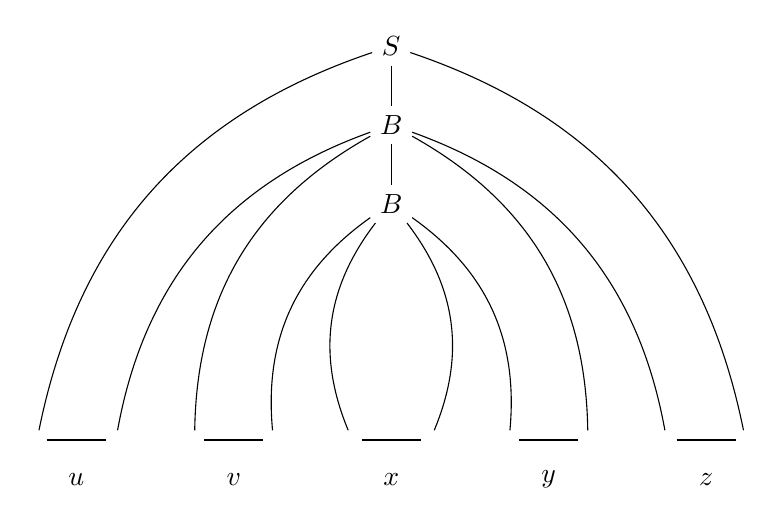
\begin{tikzpicture}[>=latex]
		% Nodes
		\node (u1) at (0,0) {};
		\node (u) at (0.5,-0.5) {$u$};
		\node (u2) at (1,0) {};
		\node (v1) at (2,0) {};
		\node (v) at (2.5,-0.5) {$v$};
		\node (v2) at (3,0) {};
		\node (x1) at (4,0) {};
		\node (x) at (4.5,-0.5) {$x$};
		\node (x2) at (5,0) {};
		\node (y1) at (6,0) {};
		\node (y) at (6.5,-0.5) {$y$};
		\node (y2) at (7,0) {};
		\node (z1) at (8,0) {};
		\node (z) at (8.5,-0.5) {$z$};
		\node (z2) at (9,0) {};

		% Upper nodes
		\node (B2) at (4.5,3) {$B$};
		\node (B1) at (4.5,4) {$B$};
		\node (S) at (4.5,5) {$S$};

		% Lines going down
		\draw[-] (B1) to (B2);
		\draw[-] (S) to (B1);


		% Lines going to terminals
		\draw[-] (B2) to[bend right] (x1);
		\draw[-] (B2) to[bend left] (x2);
		\draw[-] (x1) to (x2);

		\draw[-] (B1) to[bend right] (v1);
		\draw[-] (B2) to[bend right] (v2);
		\draw[-] (v1) to (v2);

		\draw[-] (B1) to[bend left] (y2);
		\draw[-] (B2) to[bend left] (y1);
		\draw[-] (y1) to (y2);

		\draw[-] (B1) to[bend right] (u2);
		\draw[-] (S) to[bend right] (u1);
		\draw[-] (u1) to (u2);

		\draw[-] (B1) to[bend left] (z1);
		\draw[-] (S) to[bend left] (z2);
		\draw[-] (z1) to (z2);

	\end{tikzpicture}
	\caption{\label{fig:pumpelemmacfg} Gentagelse i parsetræ for CFG}
\end{figure}


Vi kigget på sproget $B = \{a^{n}b^{n}c^{n} \mid n \ge 0\}$.
Vi tager følgende skridt:
\begin{itemize}
	\item Vi tager $w = a^{p}b^{p}c^{p}$
	\item Modstanderen viser $w = uvxyz$ hvor $|vy| > 0$ og $|vxy| \le p$
	\item Vi påstår at $uv^{0}xy^{0}z = uxz \notin L$
	\item Da $|vxy| \le p$ kan vi ikke have både $a$ og $c$ i $vxy$.
	\item Vi kigger på to muligheder præcist:
	      \begin{itemize}
		      \item $vxy \in a^{p}b^{p}$ så er $uxz \notin L$ da den har flere $C$'er end $a$'er eller $b$'er.
		      \item $vxy \in b^{p}c^{p}$ er på samme måde som før, men hvor der ville være flere $a$'er.
	      \end{itemize}
\end{itemize}




%%% Local Variables:
%%% mode: latex
%%% TeX-engine: xetex
%%% TeX-command-extra-options: "-shell-escape"
%%% TeX-master: "main"
%%% End:
